\chapter{Meteorological Data} \label{app:meteo}


% \begin{sidewaysfigure}[ht]
\rotatebox{90}{\begin{minipage}{0.8\textheight}
	\centering
    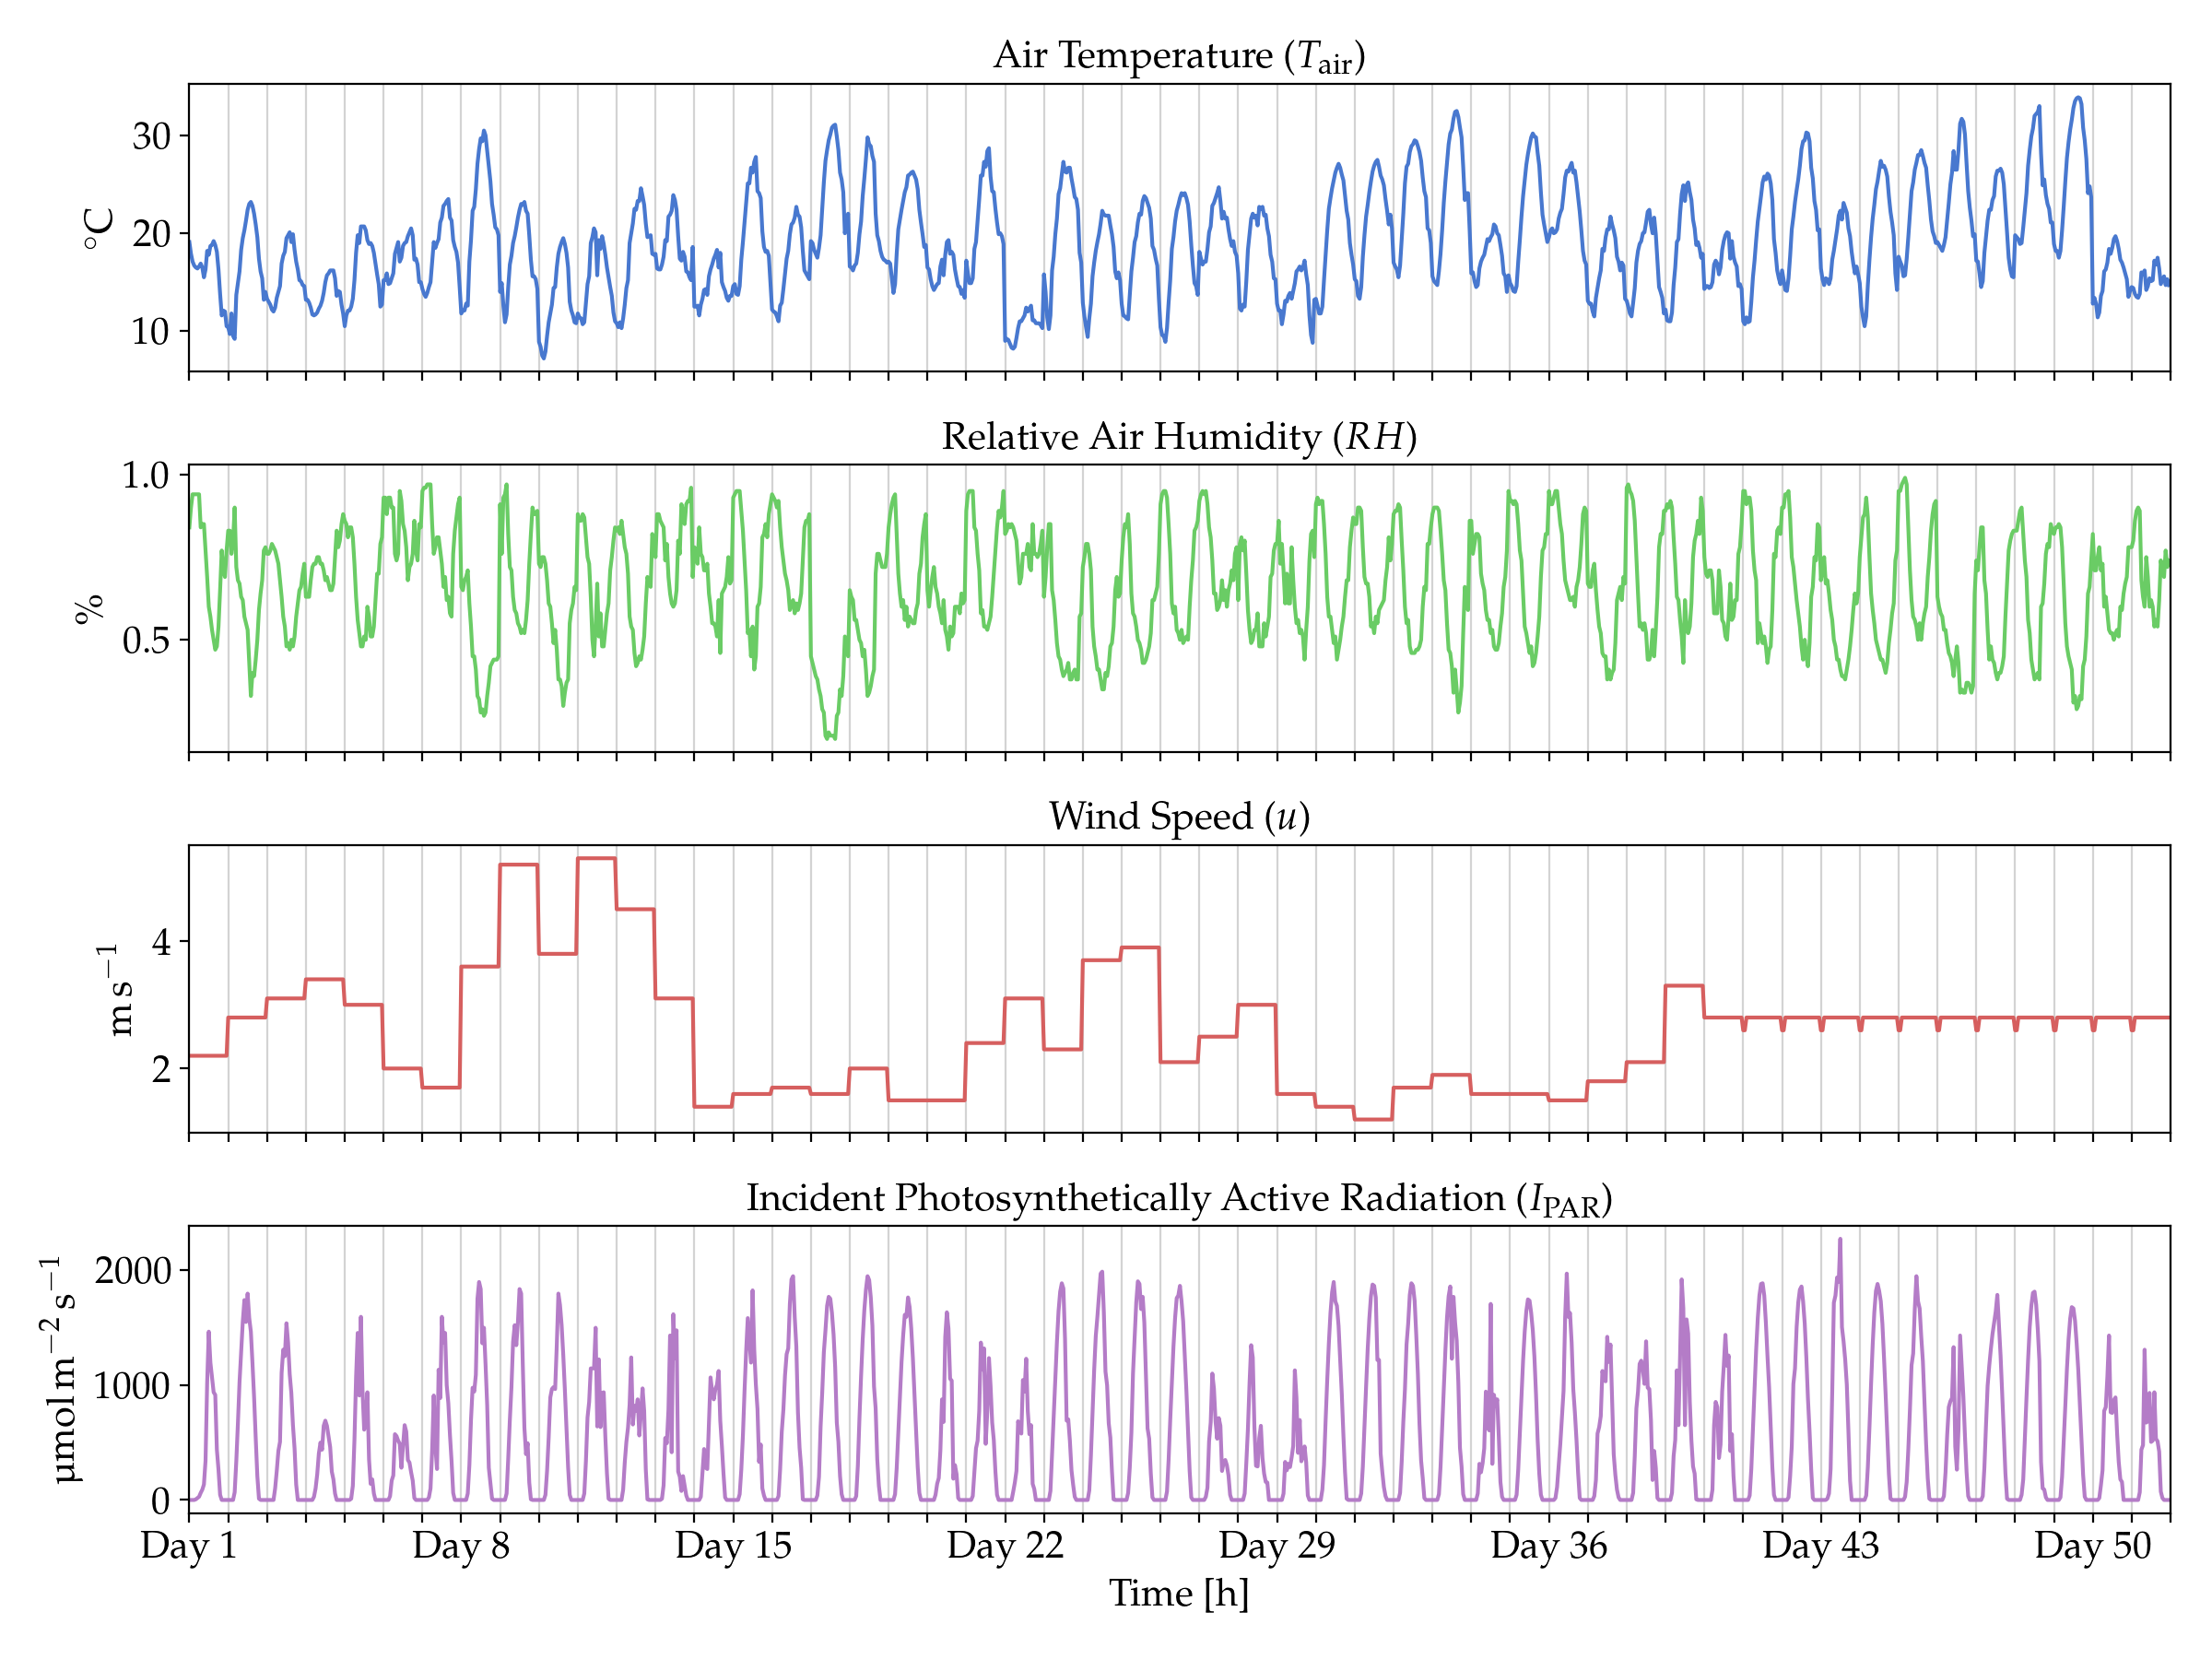
\includegraphics[width=\textwidth]{img/cn_inputs.png}
	\captionof{figure}[Hourly meteorological inputs used in CN-Wheat simulations.]
	    {
	    Hourly meteorological inputs used in CN-Wheat simulations.
	    The data was recorded in Clermont-Ferrand in central France. 
	    The data is a reconstruction of various dates in 2005.
	    See \citet{barillot_cn-wheat_2016-1} for more details.
    }
	\label{fig:cnwheat-meteo}
\end{minipage}}
% \end{sidewaysfigure}

\begin{sidewaysfigure}[ht]
	\centering
    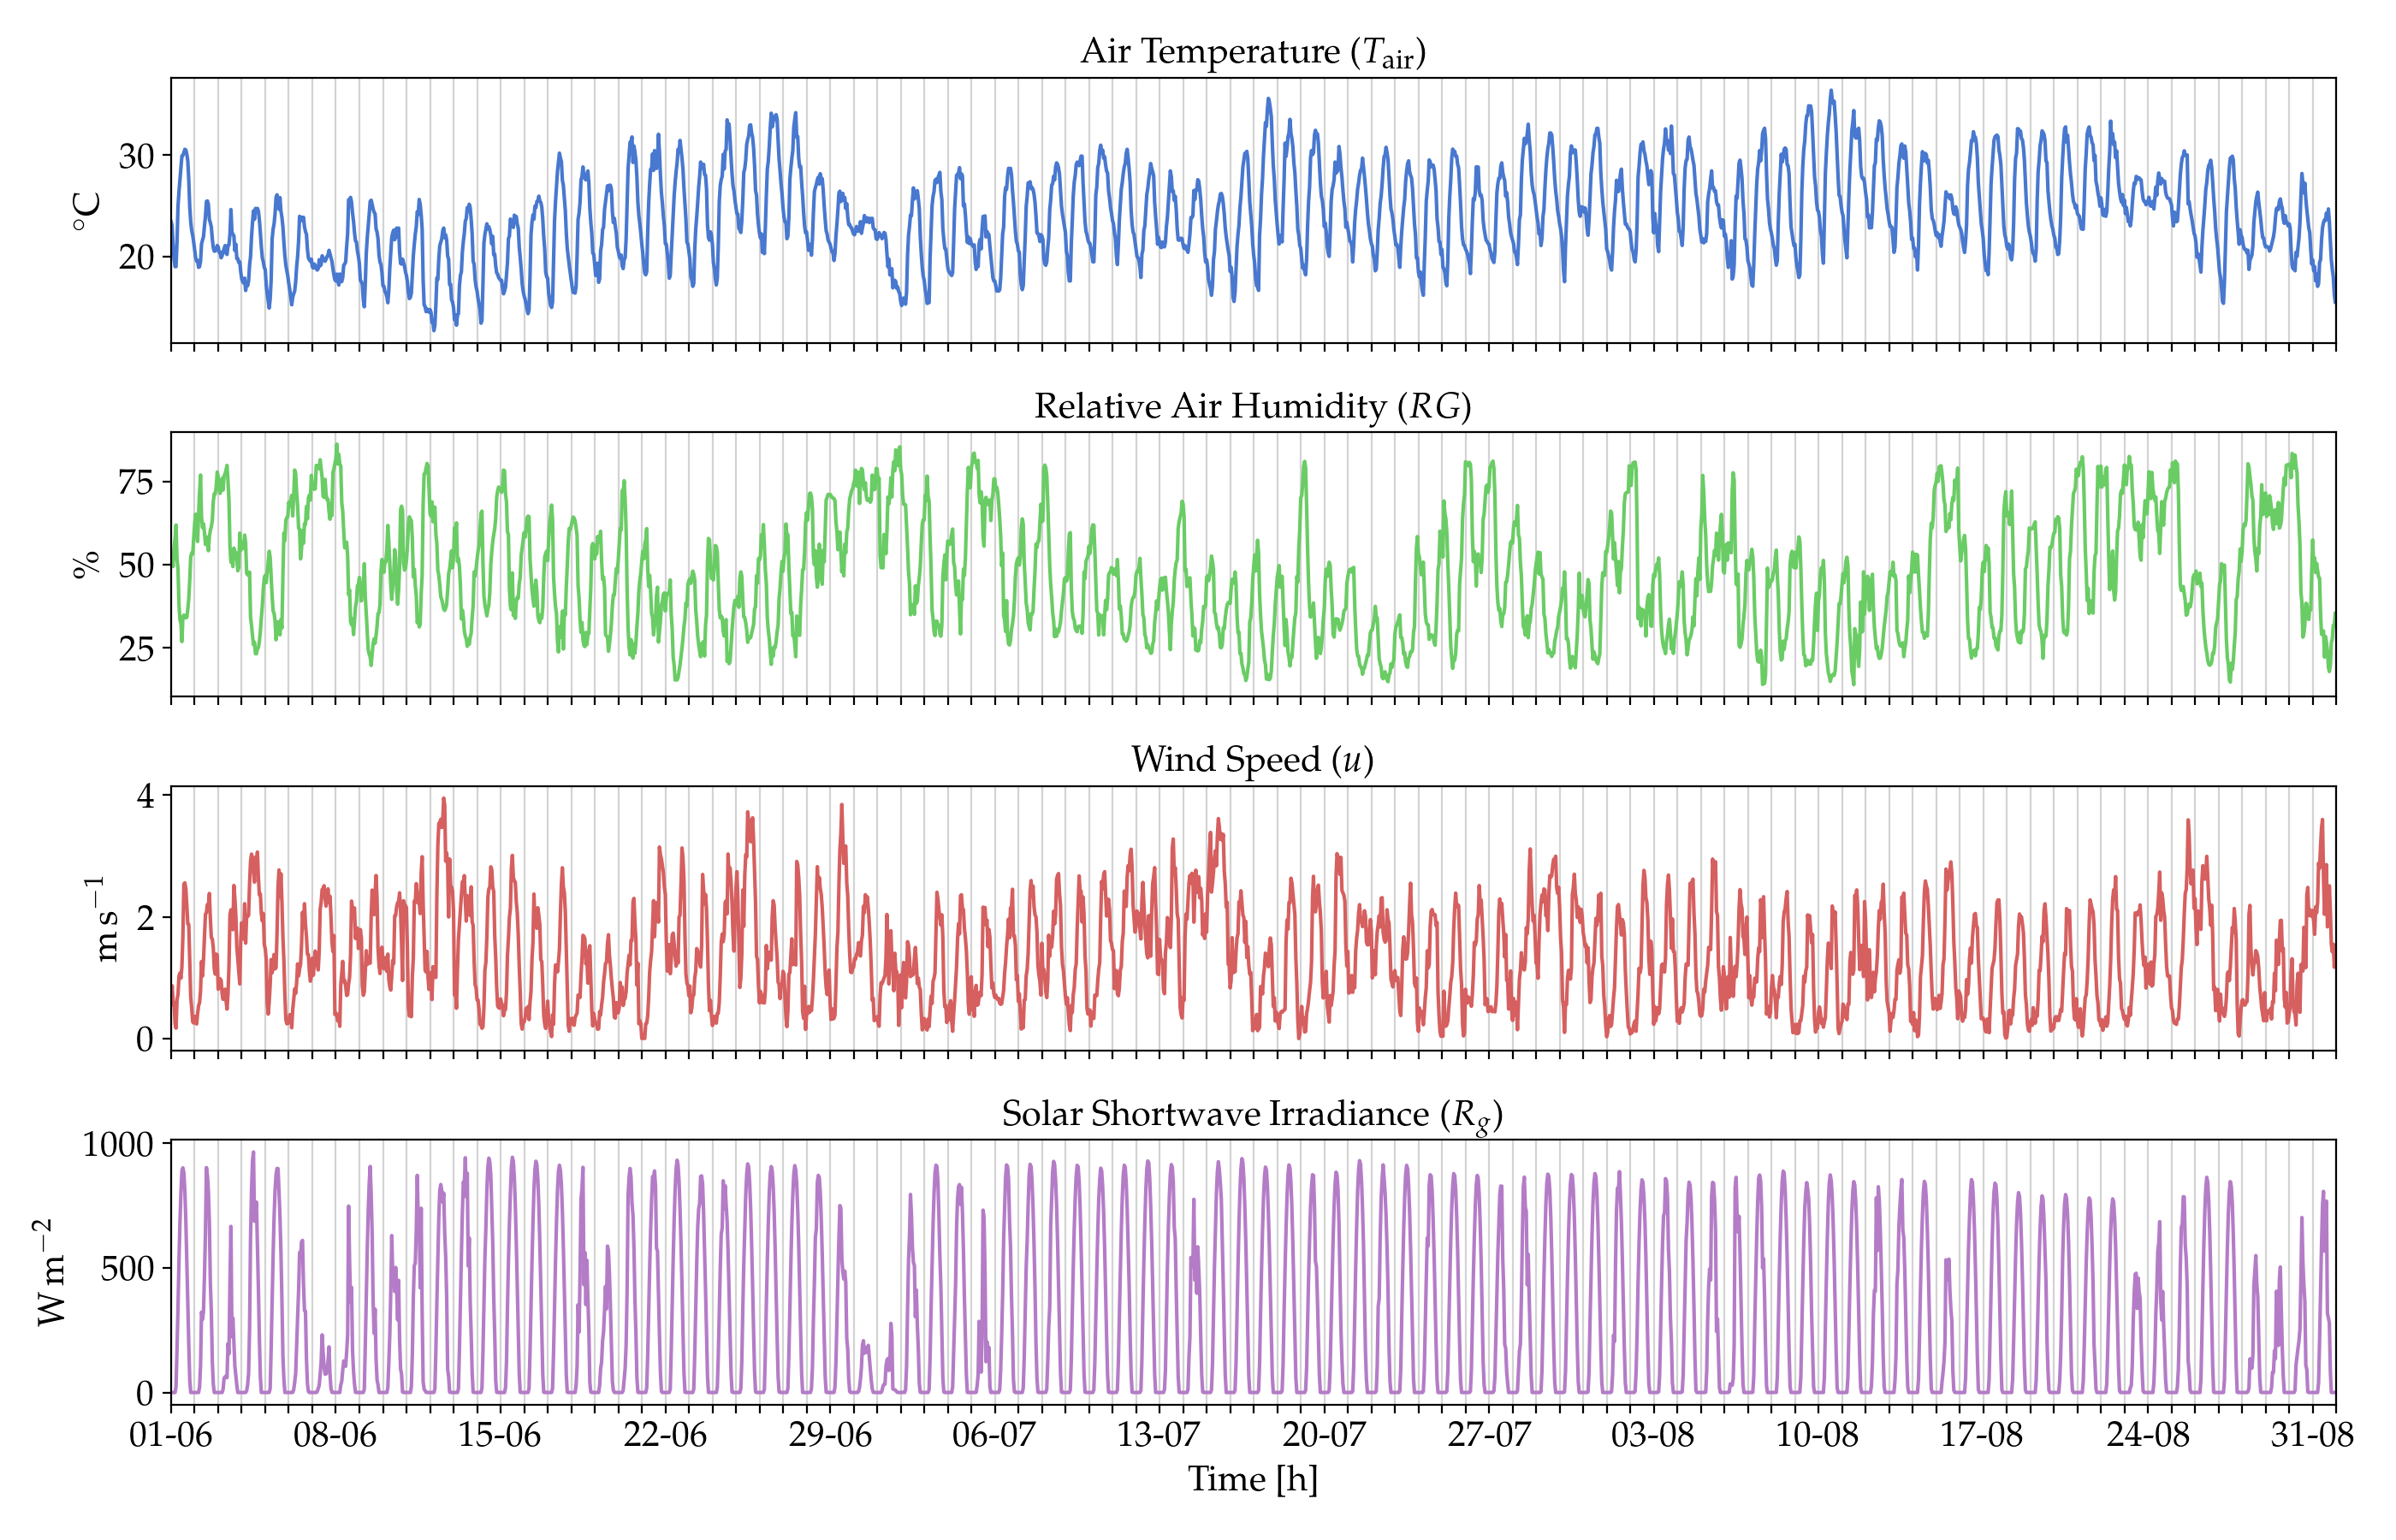
\includegraphics[width=\textwidth]{img/hs_inputs.png}
	\caption
	[Hourly meteorological inputs used in HydroShoot simulations.]
	{
	    Hourly meteorological inputs used in HydroShoot simulations.
	    The data originates from Montpellier, southern France and was recorded in 2012.
	    See \citet{albasha_hydroshoot_2019} for more details.
    }
	\label{fig:hydroshoot-meteo}
\end{sidewaysfigure}

